\documentclass{article}

\usepackage{graphicx}
\usepackage[hidelinks]{hyperref}
\usepackage[a4paper, total={6in, 8in}]{geometry}
\usepackage[slovak]{babel}
\usepackage{caption}
\usepackage{subcaption}

\graphicspath{./include/}

\renewcommand{\figurename}{Obr.}
\renewcommand{\contentsname}{Obsah}

\begin{document}

\begin{titlepage}
	\null\vfill

	\begin{center}
		{\Huge Dvojpolohová regulácia teploty tepelného systému }
		\vskip 2cm

		{\Large Cvičenie č. 9}
		\vskip 0.5cm

		{\large Spojité procesy}
	\end{center}

	\vfill
	\vfill

	\begin{flushright}
		Filip Lobpreis \\
		Matúš Machata \\
		\small\today\\
	\end{flushright}
	\hfill
\end{titlepage}

\thispagestyle{empty}
\clearpage

\tableofcontents
\thispagestyle{empty}
\clearpage

\section{Zadanie}
\label{sec:zadanie}
\pagenumbering{arabic}

\begin{figure}[!htbp]
	\begin{center}
		\label{fig:zadanie}
		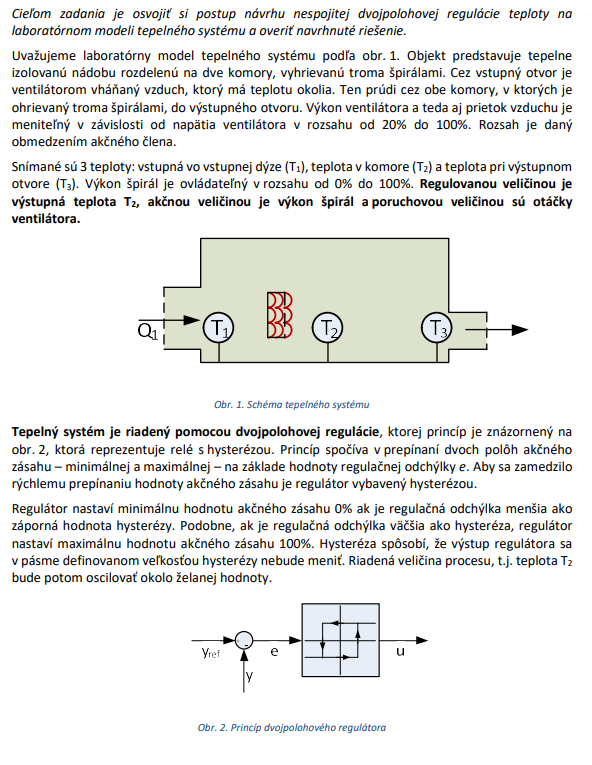
\includegraphics[width=0.8\textwidth]{./include/zadanie.png}
	\end{center}
	\caption{Zadanie z cvičenia č. 9 z predmetu spojité procesy}
\end{figure}

\clearpage

\section{Pomôcky}
\label{sec:pomocky}

V tomto zadaní je našou úlohou od simulovať návrh nespojitej dvojpolohovej regulácie teploty na laboratórnom
modeli tepelného systému a overiť navrhované riešenie. Pri tomto zadaní sme použili už preddefinovanú schému
v programe \textit{Simulink} (Obr.~\ref{fig:schema}).

\begin{figure}[!htbp]
	\begin{center}
		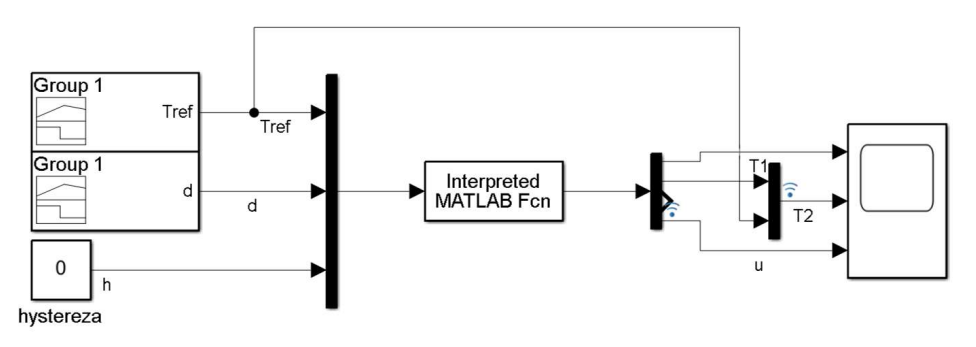
\includegraphics[width=0.95\textwidth]{./include/schema.png}
		\label{fig:schema}
		\caption{Simulacna schema reprezentujuca dvojpolohovu regulaciu tepelneho systemu.}
	\end{center}
\end{figure}

V tomto zapojení vidíme tri vstupné signály, tie sú už preddefinované. \textbf{Tref} (referenčná teplota)
má nasledujúci priebeh (viď Obr.~\ref{fig:ziadanaHodnota}).

\begin{figure}[!htbp]
	\begin{subfigure}{0.5\textwidth}
		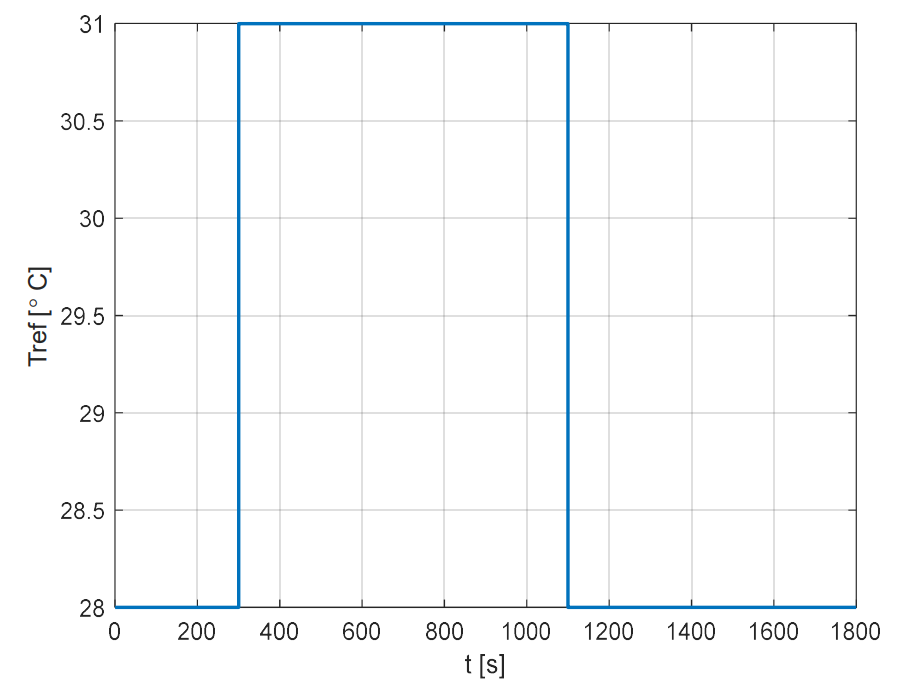
\includegraphics[width=\textwidth]{./include/ziadanaHodnota.png}
		\label{fig:ziadanaHodnota}
		\caption{Priebeh referenčnej teploty v priebehu 1800 sekúnd.}
	\end{subfigure}
	\hfill
	\begin{subfigure}{0.5\textwidth}
		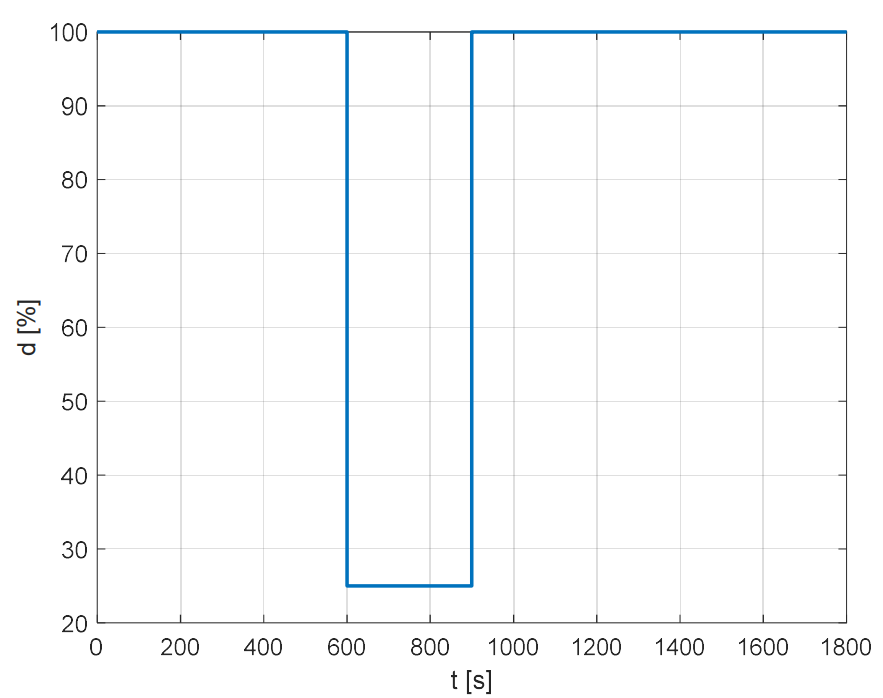
\includegraphics[width=\textwidth]{./include/porucha.png}
		\label{fig:porucha}
		\caption{Priebeh poruchy systému v priebehu 1800 sekúnd.}
	\end{subfigure}
\end{figure}

Signál \textbf{d} reprezentuje poruchu systému. Poruchovou veličinou sú otáčky ventilátora, ktoré sú závislé
od napätia na ventilátore. Toto napätie sa pohybuje v rozsahu od 20\% do 100\% (Obr.~\ref{fig:porucha}).

\section{Merania}
\label{sec:merania}

\subsection{Hysteréza s hodnotou 0,2}
\label{sec:meranie1}

V prvom zadaní sme zvolili hodnotu hysterézy 0,2. Výsledok simulácie môžeme vidieť na obrázkoch
Obr.~\ref{fig:m1t2} a Obr.~\ref{fig:m1u}.

\begin{figure}[!htbp]
	\begin{center}
		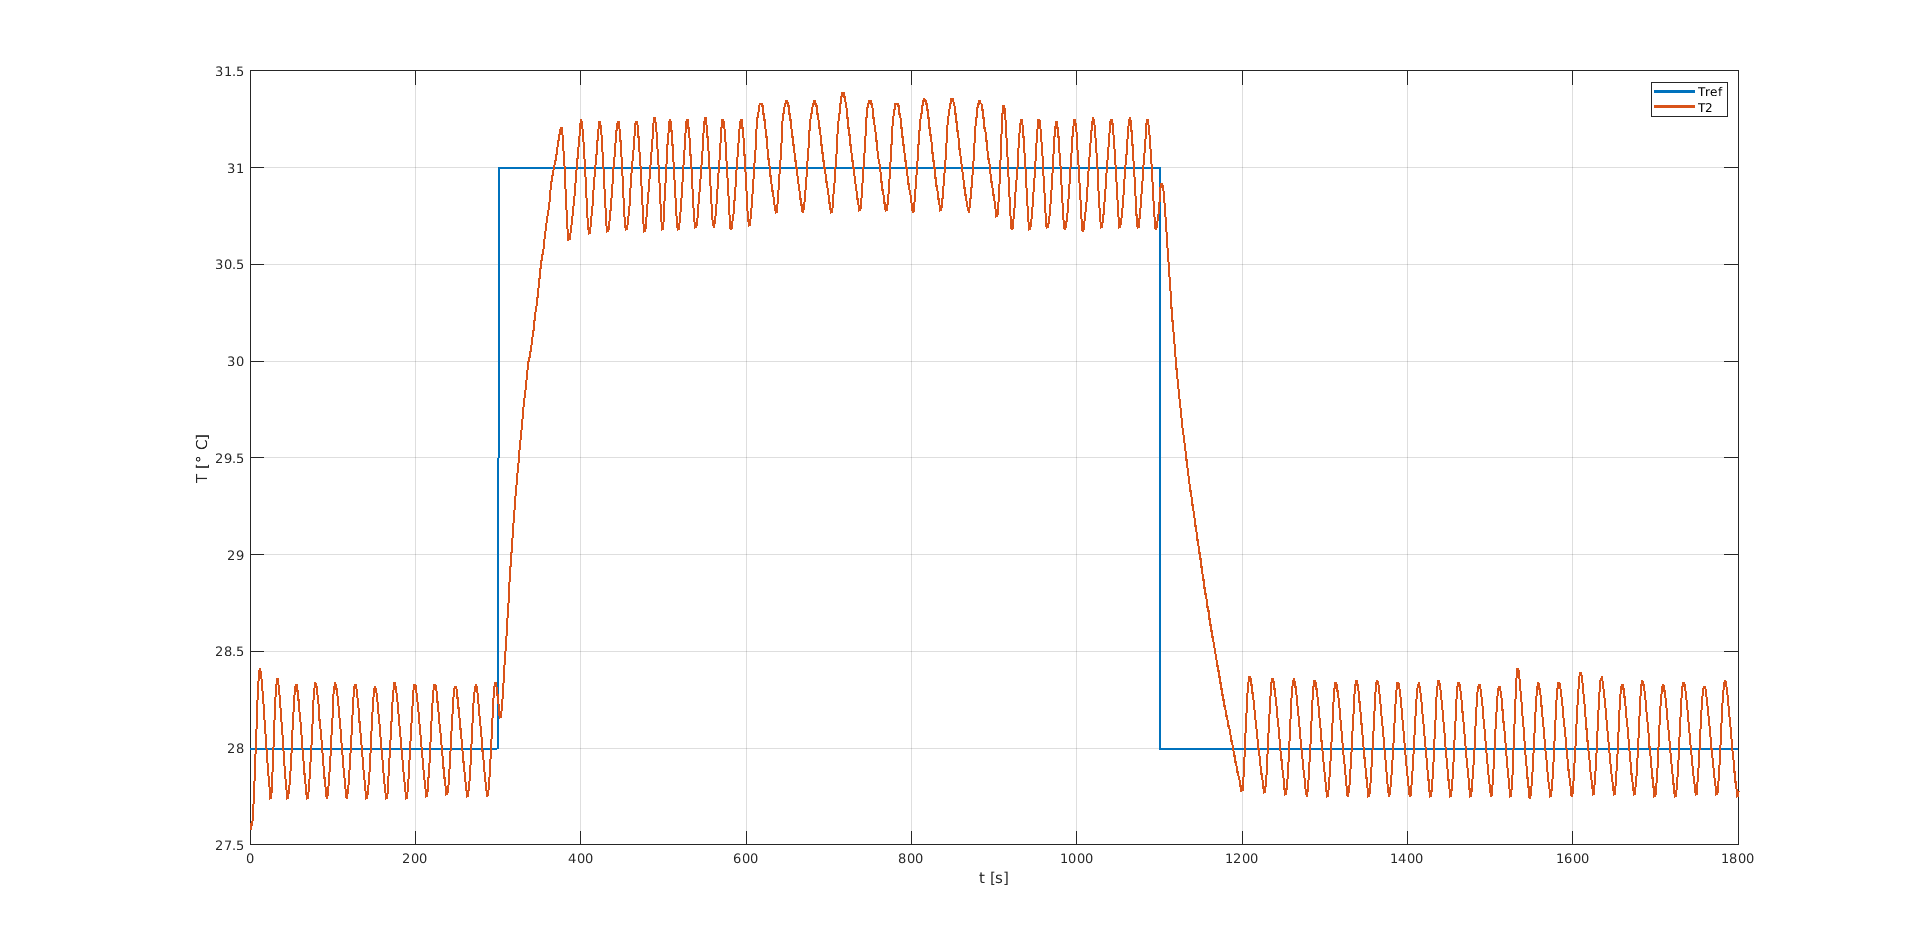
\includegraphics[width=\textwidth]{./include/m1T2.png}
	\end{center}
	\caption{Graf žiadanej a meranej hodnoty teploty na snímači T2 v prvom meraní [°C].}
	\label{fig:m1t2}
\end{figure}

\clearpage

\begin{figure}[!htbp]
	\begin{center}
		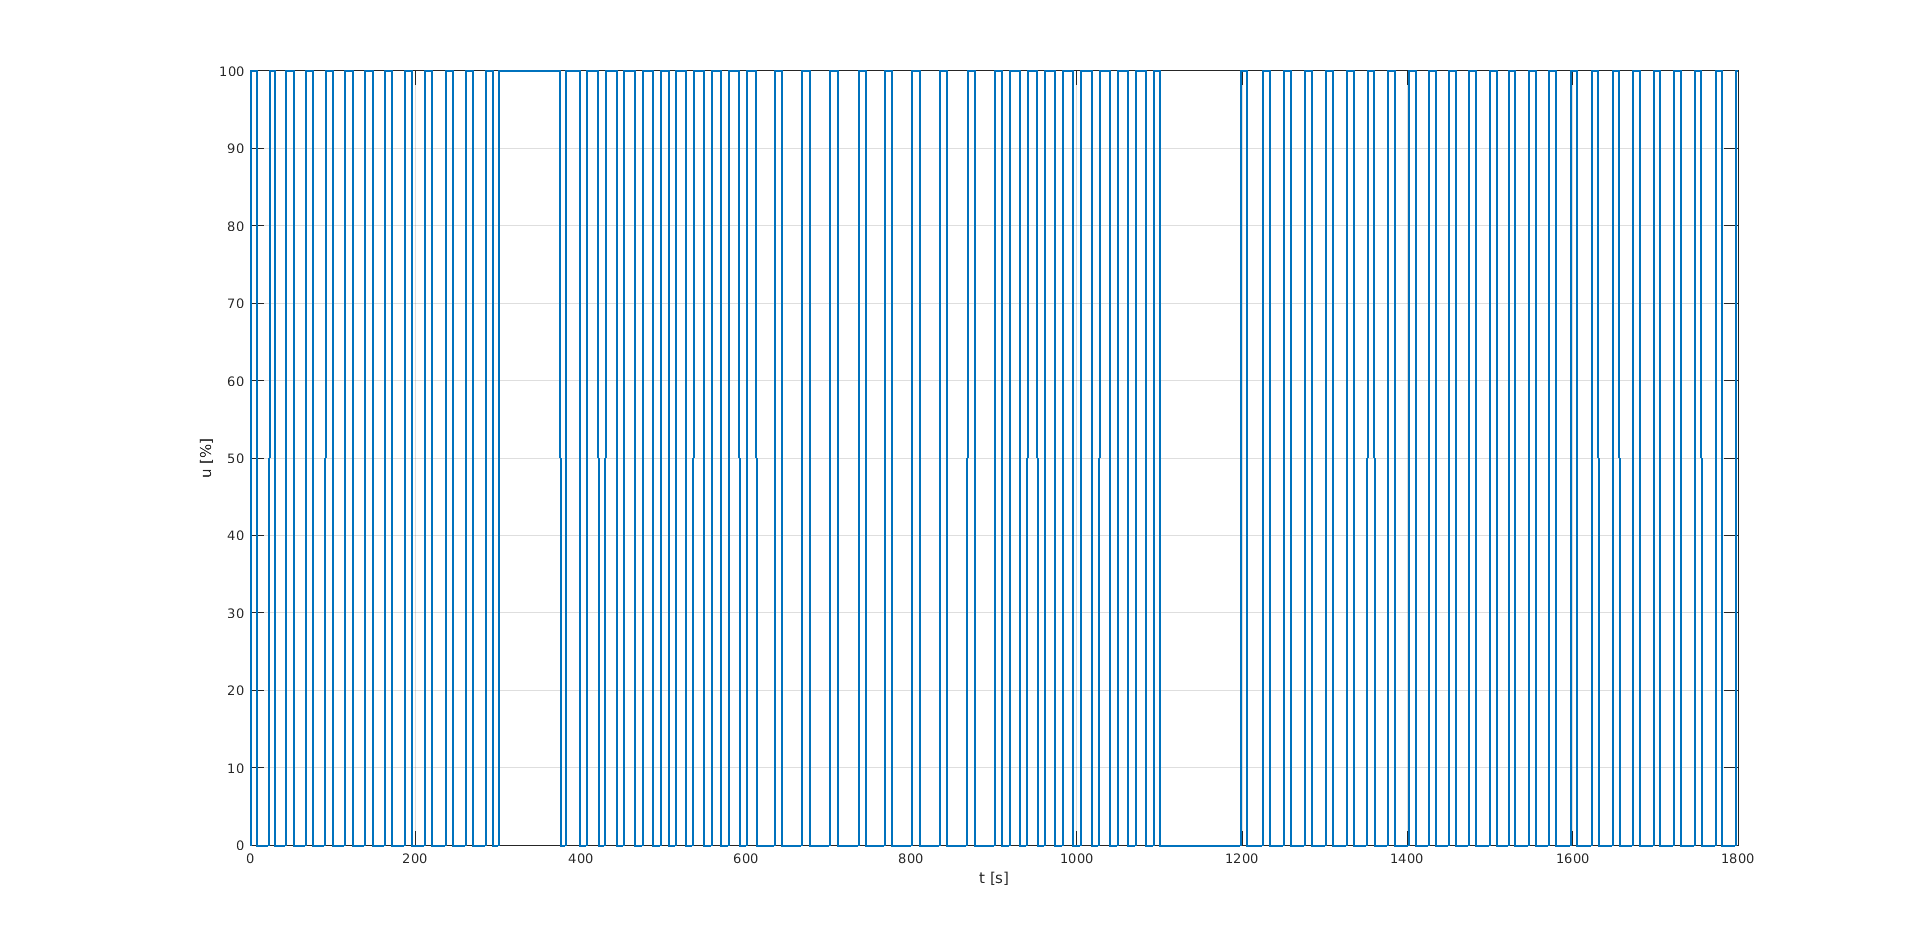
\includegraphics[width=\textwidth]{./include/m1u.png}
	\end{center}
	\caption{Graf výkonu výhrevnej špirály v prvom meraní [\%].}
	\label{fig:m1u}
\end{figure}

V prvej časti merania (od času 0s po 300s) máme žiadanú teplotu 28°C s ventilátorom zapnutým na 100\%.
V druhej časti merania (od času 300s po 600s) máme žiadanú teplotu 31°C s ventilátorom zapnutým na 100\%.
V tretej časti merania (od času 600s po 900s) máme žiadanú teplotu 31°C s ventilátorom zapnutým na 25\% a
v poslednej časti merania (od času 900s po 1800s) má systém vertikálne investované správanie ako prvé
dve časti merania. Systém ma žiadanú hodnotu teploty nastavenú na 31°C a ventilátor je zapnutý na 100\%
a prechádza do stavu, kde je žiadaná hodnota teploty 28°C a ventilátor zostane zapnutý na 100\%.
Priebeh teploty na snímači \textit{T2} vidíme na Obr.~\ref{fig:m1t2} a priebeh výkonu výhrevnej špirály
môžeme vidieť na obrázku Obr.~\ref{fig:m1u}. Spôsob správania výhrevnej špirály je opísaný v zadaní.
\ref{sec:zadanie}.

\clearpage

\subsection{Hysteréza s hodnotou 0,5}
\label{sec:meranie2}

\begin{figure}[!htbp]
	\begin{center}
		\includegraphics[width=\textwidth]{./include/m2T2.png}
	\end{center}
	\caption{Graf žiadanej a meranej hodnoty teploty na snímači T2 v druhom meraní [°C].}
	\label{fig:m2t2}
\end{figure}

\clearpage

\begin{figure}[!htbp]
	\begin{center}
		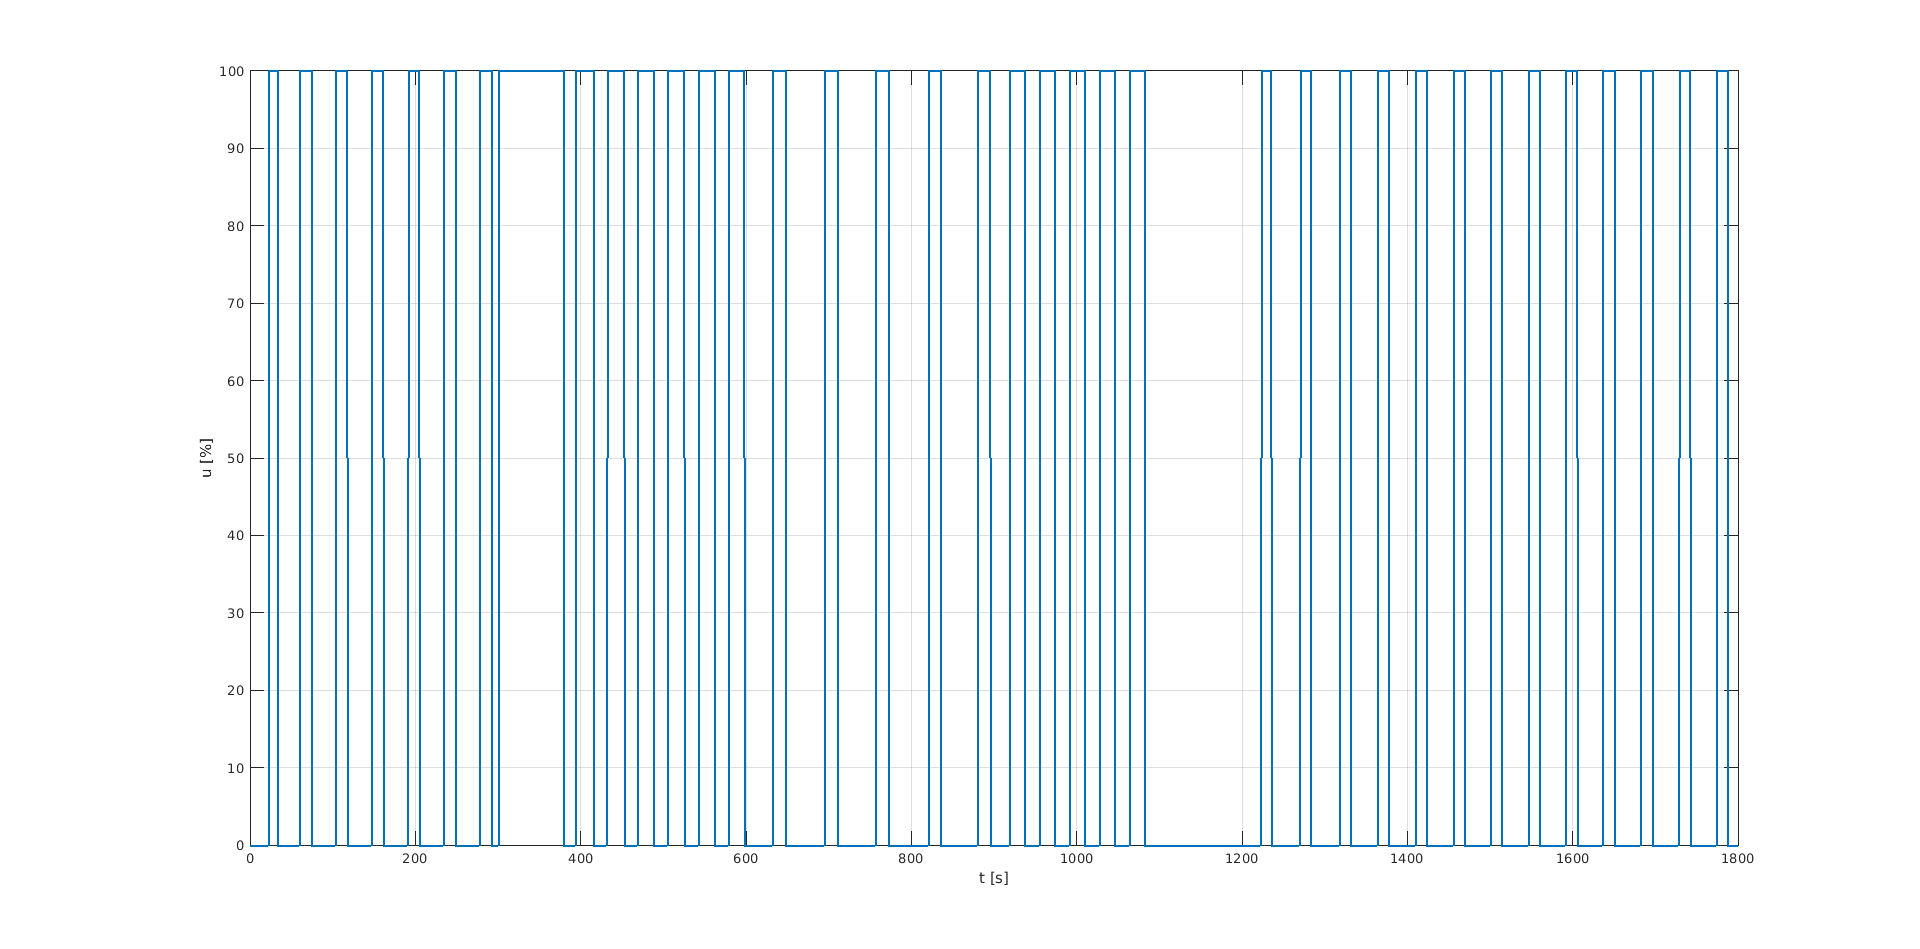
\includegraphics[width=\textwidth]{./include/m2u.png}
	\end{center}
	\caption{Graf výkonu výhrevnej špirály v druhom meraní [\%].}
	\label{fig:m2u}
\end{figure}

V druhom meraní máme zvolenú hodnotu hysterézy 0,5. Rozdelenie časti simulácie je rovnaké ako v prvom meraní.
Rozdiel nastáva v responzívnosti systému na zmenu teploty. V druhom meraní je responzívnosť systému menšia
kvôli už spomínanej vyššej hodnote hysterézy. Ako môžeme vidieť na obrázku Obr.~\ref{fig:m2t2}, frekvencia
meranej teploty na snímači T2 je menšia a zároveň aj strmosť tejto zmeny je menšia.

\subsection{Hysteréza s hodnotou 0,8}
\label{sec:meranie3}

\begin{figure}[!htbp]
	\begin{center}
		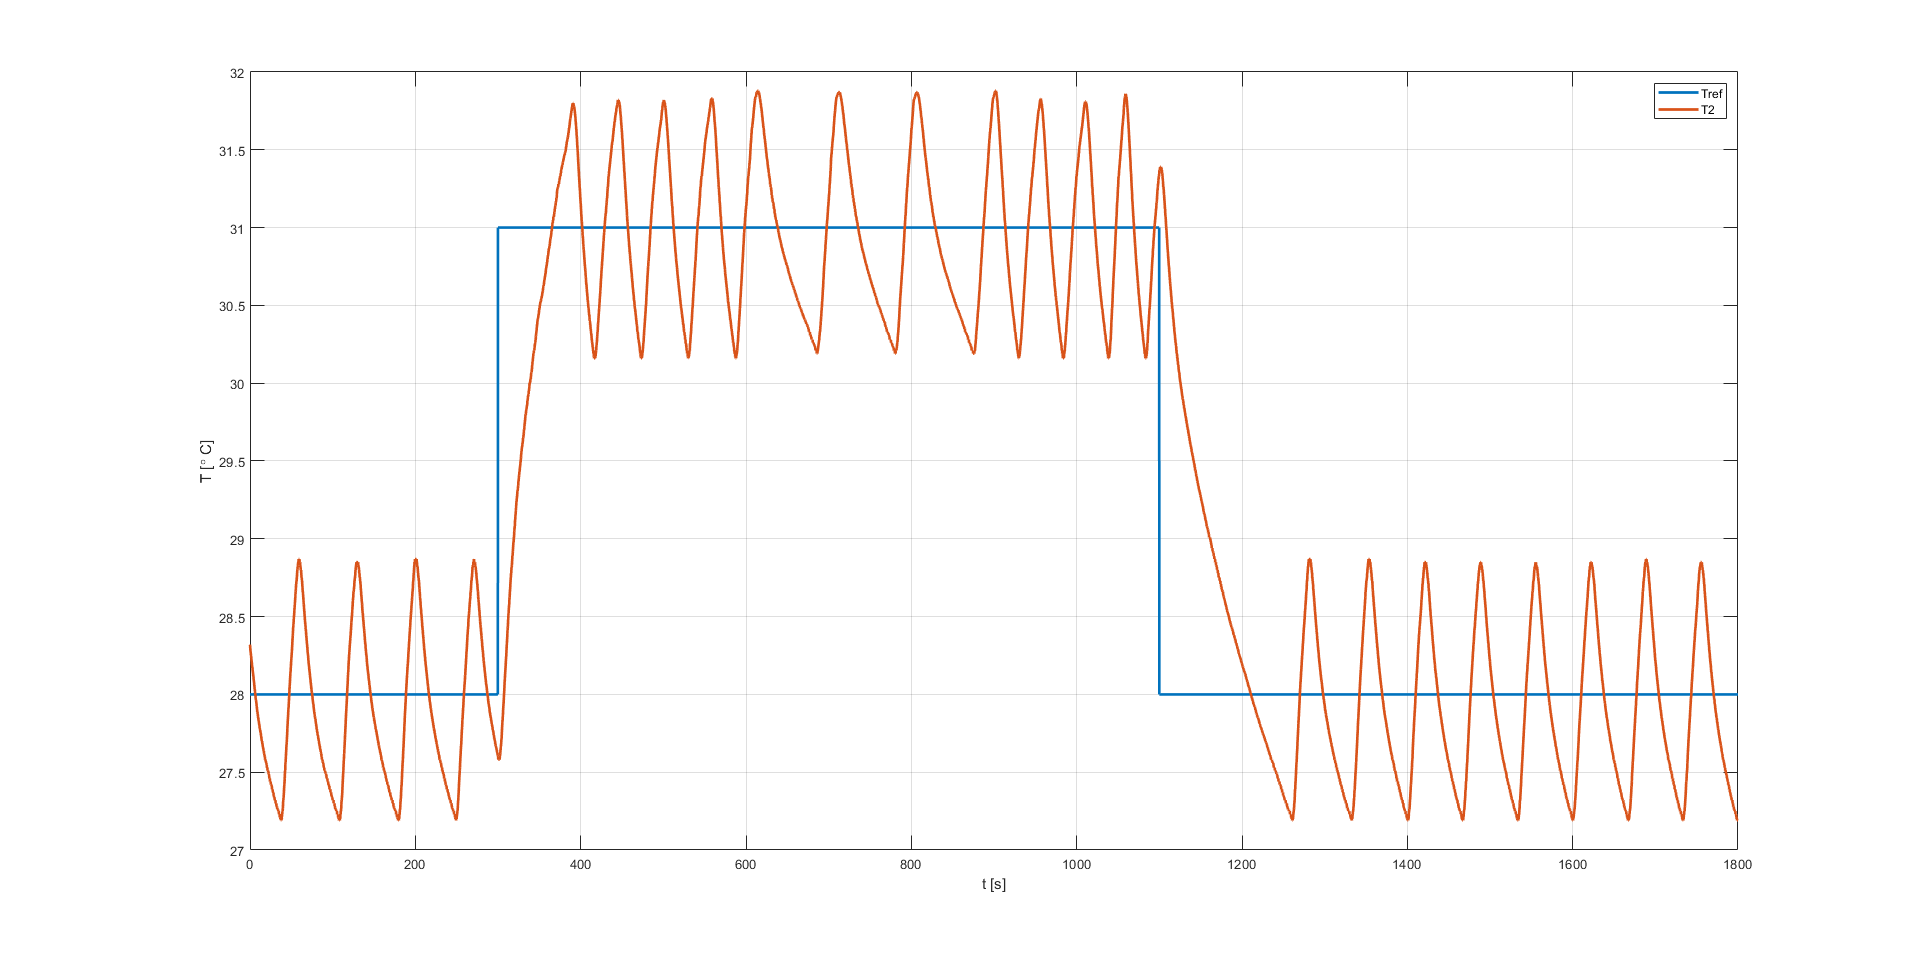
\includegraphics[width=\textwidth]{./include/m3T2.png}
	\end{center}
	\caption{Graf žiadanej a meranej hodnoty teploty na snímači T2 v treťom meraní [°C].}
	\label{fig:m3t2}
\end{figure}

\clearpage

\begin{figure}[!htbp]
	\begin{center}
		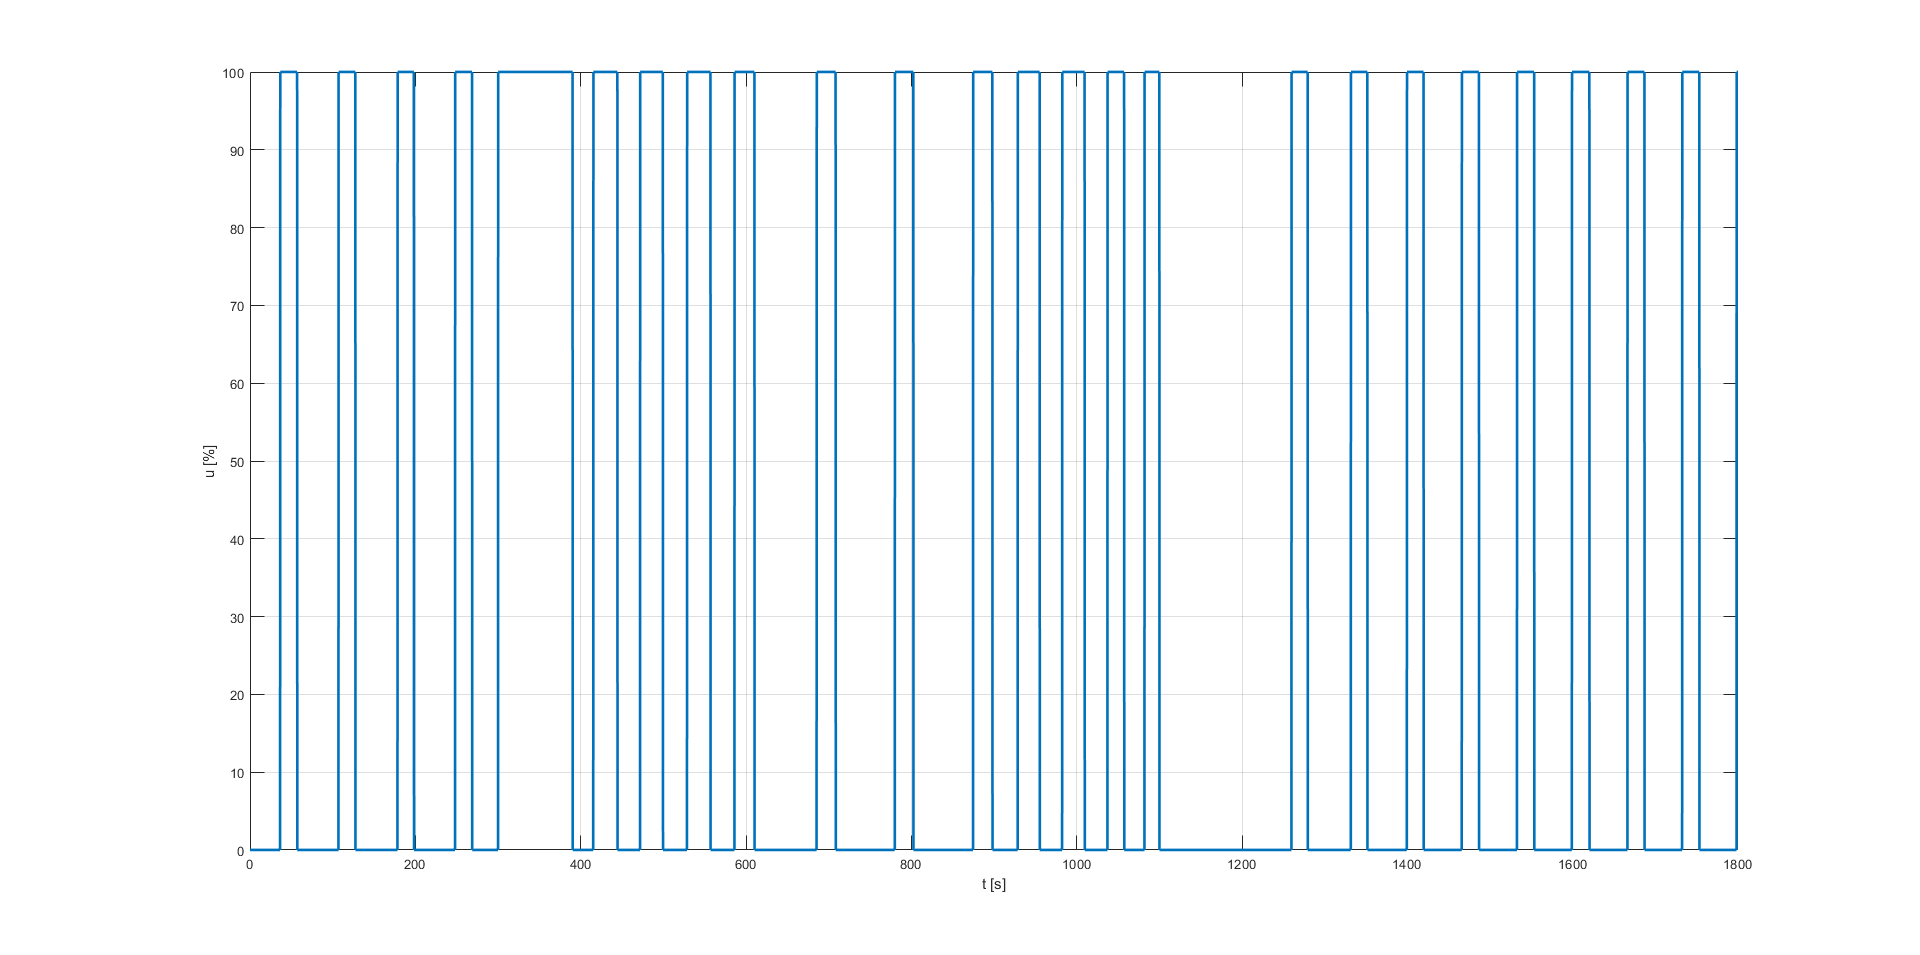
\includegraphics[width=\textwidth]{./include/m3u.png}
	\end{center}
	\caption{Graf výkonu výhrevnej špirály v treťom meraní [\%].}
	\label{fig:m3u}
\end{figure}

Tak isto ako pri druhom meraní, frekvencia a strmosť zmeny teploty T2 sa zmenšili kvôli zvýšeniu hodnoty hysterézy čo môžeme vidieť na Obr.~\ref{fig:m3t2}. Preto sa aj perióda zapínania výhrevnej špirály zmenšila ako môžeme vidieť na Obr.~\ref{fig:m3u}.

\section{Zhrnutie}
\label{sec:zhrnutie}

V tomto zadaní sme zisťovali dôsledok zmeny hodnoty hysterézy na teplotu T2. Na obrázkoch () sme pozorovali nasledujúce správanie. Čím je hodnota hysterézy menšia, tým máme menšiu periódu zapínania, resp. vypínania ohrievacej špirály. Zároveň sme mohli vidieť zmenu strmosti zmeny teploty na snímači T2. Túto strmosť a taktiež aj frekvenciu ovplyvňuje aj vypnutie ventilátora, čo si môžeme všimnút v čase od 600s po 900s na každej simulácii v už spomínaných obrázkoch. Hodnota hysterézy teda ovplyvňuje dvojpólovú reguláciu výstupnej teploty. ak nám záleží na najpresnejšom udržiavaní žiadanej hodnoty, tak sa nám oplatí zvoliť si menšiu hodnotu hysterézy. Naopak ak chceme dosiahnuť čo najmešie zaťaženie ohrievacej špirály tak je vhodné zvoliť si väčšiu hodnotu hysterézy.


\end{document}

